\chapter{Background}\label{Ch:Background}
This chapter establishes the theoretical and geological foundations upon which this research is built. 
It provides a comprehensive overview of the geological setting of the Delft reservoir and a literature review of modern geomodelling and machine learning (ML) techniques.
Section~\ref{Sec:Delft_Reservoir} introduces the geological context of the Delft reservoir, detailing its depositional environment and current conceptual model. 
Section~\ref{Sec:Geomodelling} explores the state-of-the-art in geological modelling, comparing traditional techniques and their respective limitations. 
Finally, Section~\ref{Sec:ML} provides an in-depth review of machine learning and deep learning (DL) principles, focusing on their historical evolution and contemporary application to subsurface characterization. 
This balanced overview is intended to provide both geological and computer science readers with the necessary context to understand the research methodology and results presented in subsequent chapters.

%=====================================================================================%
% Chapter outline:  
%    - General Introduction of the 
%       - Geology of the Delft reservoir
%           - West Netherlands Basin
%           - Reservoir stratigraphy and sedimentology
%           - Current geological conceptual model
%       - Current geomodelling practises
%           - Modelling approaches
%           - conditioning
%       - Machine Learning
%           - Deep learning
%           - ML in the subsurface
%       - Summary
%=====================================================================================%
\section{The Delft Geothermal Reservoir}\label{Sec:Delft_Reservoir}
The data utilized in this study is sourced from the Delft geothermal reservoir, situated beneath the \gls{tud} Campus in the Netherlands. 
As of February 2026, a geothermal doublet is actively producing heat from this reservoir~\parencite{beerda2026geothermie}. 
A doublet system consists of a two-well setup: a producer well extracts warm formation water, and an injector well returns the cooled water to the reservoir. 
At the Delft site, the producer well (\textbf{DEL-GT-01}) was drilled to a \gls{tvd} of approximately 2,337~m, while the injector well (\textbf{DEL-GT-02-S2}) reached a \gls{tvd} of approximately 2,100~m~\parencite{vardon2024endofwell}. 
The project serves both commercial and research objectives, acquiring extensive geophysical logs and core data, supplemented by surface and downhole monitoring instrumentation~\parencite{vardon2020geothermal, vardon2024endofwell}.
Despite the high data density, the cored section is restricted to the first 80~m of the \textbf{DEL-GT-01} well (approximately one-fourth of the reservoir thickness), while \textbf{DEL-GT-02-S2} contains no cored sections.
The primary target is the \gls{dsst}, a member of the Lower Cretaceous Nieuwerkerk Formation in the \gls{wnb}~\parencite{donselaar2015reservoir}.

\subsection{Geology of the Delft Reservoir}
The \gls{wnb} is a 60~km wide transtensional basin in the southwest of the Netherlands, characterized by NW-SE trending structural highs and depressions~\parencite{ziegler1990geological, donselaar2015reservoir}. 
The \gls{wnb} entered an active rifting stage during the Middle Jurassic~\parencite{bodenhausen1981habitat, den1996fluviomarine, willems2020geology}, leading to the formation of several half-grabens filled with terrestrial sediments sourced from neighboring regions~\parencite{den1996fluviomarine}. 
The progressive filling of these half-grabens coincided with a change in the depositional environment as a transgressive shoreline moved the system from fluvial to marine. 
The Nieuwerkerk Formation comprises three members: the Alblasserdam, the \gls{dsst}, and the Rodenrijs Claystone. 

The Alblasserdam member was deposited in a fluvial environment characterized by stacked channels and floodplain deposits~\parencite{devault2002tectonostratigraphy}. 
The \gls{dsst} directly overlays the Alblasserdam and consists of thick, stacked fluvial-deltaic channel sandstones with high net-to-gross values, oriented NW-SE~\parencite{willems2020geology, mijnlieff2020introduction, bruining2023sedimentological, groenenberg2010targeting}. 
The \gls{dsst} is in turn overlain by the Rodenrijs Claystone, an organic-rich lagoonal deposit~\parencite{willems2020geology, devault2002tectonostratigraphy, bruining2023sedimentological}.

Based on the sedimentological analysis of the \textbf{DEL-GT-01} core and \textbf{DEL-GT-02-S2} sidewall samples, three primary facies associations (FAs) have been identified~\parencite{bruining2023sedimentological}:
\begin{itemize}
    \item \textbf{FA1: Fluvial and distributary channel deposits.} Primarily light grey, fine- to medium-grained sandstones featuring low-angle cross-bedding and ripple lamination, with unit thicknesses ranging from 5 to 80~m. 
    \item \textbf{FA2: Crevasse splays and levee deposits.} Composed of moderately sorted, very fine- to medium-grained sandstones interbedded with dark grey siltstones, with thicknesses ranging from 1 to 5~m. 
    \item \textbf{FA3: Overbank deposits and paleosols.} Consists of dark grey siltstones, claystones, and very fine-grained sand deposited in low-energy environments. This association is characterized by abundant organic material, slickensides, and siderite nodules.
\end{itemize}

The specific depositional environment of the \gls{dsst} remains a subject of scientific discussion. 
It has been attributed to both fluvial-meandering~\parencite{donselaar2015reservoir, vondrak2018reservoir, willems2020geology} and fluvio-deltaic systems~\parencite{van1993stratigraphic, weert2024multiple, bruining2023sedimentological}. 
Recent analysis suggests that the cored section represents a deltaic environment~\parencite{bruining2023sedimentological}. 
However, due to limited core coverage, it is hypothesized that the lower \gls{dsst} likely represents a fluvial environment, while the upper section reflects the transgressive shift toward a deltaic system.

\subsection{Deltaic Depositional Environment}
Deltaic environments form at the land-sea interface where river systems supply clastic sediments. 
Delta morphology is governed by the relative influence of fluvial, wave, and tidal processes~\parencite{kolb1966depositional}. 
The subaerial delta plain is typically divided into two domains~\parencite{kolb1966depositional, heldreich2017challenges}:
\begin{itemize}
    \item \textbf{Upper Delta Plain:} Lies above the limit of saltwater intrusion. Sedimentation is driven by distributary channel migration, overbank flooding, and crevassing. Environments include meandering and braided channels, lacustrine fills, and floodplains.
    \item \textbf{Lower Delta Plain:} Subject to river-marine interaction and tidal influence. Channels are more numerous and exhibit bifurcating or anastomosing patterns. Interdistributary bays, bay fills (crevasse splays), and marshes dominate the landscape.
\end{itemize}

In the \gls{dsst}, FA1 features organic material and siltstones indicating slackwater periods, while the lack of bioturbation suggests high sedimentation rates. 
The fine-grained nature of FA2 and FA3 reflects more distal positions on the delta plain. 
Siderite nodules in FA3 indicate anoxic, waterlogged conditions~\parencite{samuel1959some}, while soft-sediment deformation suggests rapid loading of mudstones over saturated sands. 
These features collectively indicate that FA3 represents deposition within a delta plain, likely in an interdistributary bay or a pro-delta environment.

\begin{figure}[!h]
    \centering
    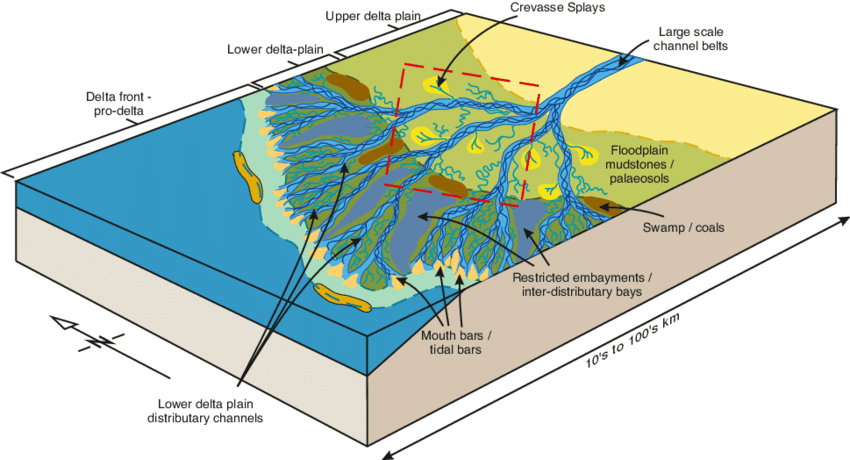
\includegraphics[width=0.85\linewidth]{figures/Upper_lower_Delta_Heldreich_2017.png}
    \caption{Depositional model of the Mungaroo Formation, illustrating the geometries and domains of a fluvial-deltaic system~\parencite{heldreich2017challenges}.}\label{fig:UpperLowerDelta}
\end{figure}

\section{Geological Modelling}\label{Sec:Geomodelling}
The primary objective of 3D reservoir modelling is to provide a representative volume of the subsurface for flow simulation and decision support. 
These models are dynamic, requiring updates as new data becomes available to refine predictions over the reservoir's lifetime~\parencite{emerick2025ensemble, ringrose2016reservoir}. 
Existing techniques are generally categorized into three types~\parencite{koltermann1996heterogeneity}:
\begin{itemize}
    \item \textbf{Geostatistical (Pixel-based) Models:} Use spatial statistics (e.g., variograms) for cell-by-cell property assignment. They are efficient and honor dense well data but often fail to capture complex connectivity, resulting in pixelated realizations.
    \item \textbf{Object-based Models:} Directly place geometric features (e.g., channels) based on geological rules. They offer high visual realism but struggle to honor dense or closely spaced well data.
    \item \textbf{Process-based Models:} Simulate the physical laws of sediment transport and deposition (conservation of mass and momentum). They provide the highest degree of realism but are computationally expensive and difficult to condition to specific hard data like well logs.
\end{itemize}
To leverage the strengths of each, hybrid models have been developed~\parencite{lopez2009process, michael2010combining}. 
Table~\ref{tab:Geomodelling_comparison} summarizes the comparison between these techniques.

\begin{table}[htbp]
    \centering
    \renewcommand{\arraystretch}{1.5}
    \begin{tabular}{p{0.18\textwidth} p{0.24\textwidth} p{0.24\textwidth} p{0.24\textwidth}}
        \hline
        \textbf{Attribute} & \textbf{Geostatistical} & \textbf{Object-Based} & \textbf{Process-Based} \\
        \hline
        \textbf{Geological Prior} & Variograms, training images. & Geometric shapes and rules. & Physical boundary conditions. \\
        \textbf{Realism} & Low to Moderate. & Moderate to High. & Very High. \\
        \textbf{Key Advantages} & Computational speed, well conditioning. & Realistic connectivity. & Physical consistency. \\
        \textbf{Key Disadvantages} & Lack of crisp shapes. & Difficult conditioning. & High computational cost. \\
        \hline
    \end{tabular}
    \caption{Comparison of spatial modelling techniques in geomodelling.}\label{tab:Geomodelling_comparison}
\end{table}

\section{Machine Learning}\label{Sec:ML} 
Machine learning (ML) involves the development of algorithms that learn patterns and inference from data to perform specific tasks without explicit programming~\parencite{goodfellow-et-al-2016}. 
The field has evolved significantly since~\textcite{samuel1959some} introduced the term, leading to diverse techniques applied across various domains. 
ML is primarily categorized into:
\begin{itemize}
    \item \textbf{Supervised Learning:} The algorithm is trained on a labeled dataset (input-output pairs). 
    \item \textbf{Unsupervised Learning:} The algorithm identifies patterns in unlabeled data without prior knowledge of the output. 
\end{itemize}
Common ML tasks include classification, regression, clustering, and generation. 
The modern state of ML is largely driven by Artificial Neural Networks (ANNs). 
Inspired by the biological structure of the brain, ANNs consist of interconnected artificial neurons that process information across multiple layers~\parencite{goodfellow-et-al-2016}. 
These networks excel at uncovering complex, non-linear relationships in vast datasets~\parencite{lecun2015deep}.

\subsection{Deep Learning and Inductive Biases}
Deep learning (DL) is a subset of ML focusing on multi-layered neural networks that represent data with multiple levels of abstraction~\parencite{goodfellow-et-al-2016, lecun2015deep}. 
Two critical concepts in DL are the ``curse of dimensionality'' and ``inductive biases.'' 
The curse of dimensionality describes the exponential increase in data required as the dimensionality grows, making high-dimensional estimation computationally challenging.

Inductive biases are architectural choices that prioritize certain outcomes, helping models generalize from limited data~\parencite{prince2023understanding}. 
Different architectures apply specific biases:
\begin{itemize}
    \item \textbf{Convolutional Neural Networks (CNNs):} Leverage spatial locality and translation invariance, making them ideal for image and 3D volume tasks. 
    \item \textbf{Recurrent Neural Networks (RNNs):} Designed for sequential data to capture temporal dependencies. 
    \item \textbf{Physics-Informed Neural Networks (PINNs):} Incorporate physical laws into the loss function to ensure consistency with scientific principles. 
\end{itemize}
A critical component of the DL workflow is the use of validation and testing protocols to prevent overfitting and ensure that learned patterns are robust and applicable to unseen data.

\subsection{Geomodelling with Deep Learning}
Integration of DL into geomodelling has evolved from simple pixel-based interpolations to sophisticated structural representations. 
DL allows for the direct learning of geological features from large datasets or process-based simulations, bridging the gap between descriptive statistics and geological realism~\parencite{laloy2017inversion}. 
CNNs have been particularly successful in identifying structural features like faults or channels from seismic and well data~\parencite{sun2023geological}. 
These techniques enable the generation of stochastic realizations that honor both the global geological concept and local conditioning data, enhancing uncertainty characterization~\parencite{song2023gansim}.

\subsection{Generative Adversarial Networks}\label{Subsec:GAN_Theory}
Generative Adversarial Networks (GANs) utilize a competitive framework between two networks~\parencite{goodfellow2014generative}: a Generator ($\mathbf{G}$) and a Discriminator ($\mathbf{D}$). 
The generator creates synthetic samples, while the discriminator attempts to distinguish them from real data. This minimax game is expressed as:
\begin{equation}
    \min_{\mathbf{G}} \max_{\mathbf{D}} V(\mathbf{D}, \mathbf{G}) = \mathbb{E}_{\mathbf{x} \sim p_{\text{data}}(\mathbf{x})}[\log \mathbf{D}(\mathbf{x})] + \mathbb{E}_{\mathbf{z} \sim p_{\mathbf{z}}(\mathbf{z})}[\log(1 - \mathbf{D}(\mathbf{G}(\mathbf{z})))]
\end{equation}
where $\mathbf{x}$ represents real data and $\mathbf{z}$ is a latent vector from a prior distribution $p_{\mathbf{z}}$. 
GANs can learn to generate high-fidelity geological realizations that capture complex features without an explicit likelihood function.
Conditional GANs (cGANs) allow auxiliary information (e.g., well logs) to steer the generation process~\parencite{mirza2014conditional}. 

Recent research has focused on improving the stability of GAN-based geomodels through refined distance metrics like the Mean Sliced Wasserstein Distance (MSWD)~\parencite{bhavsar2024stable}. 
MSWD projects high-dimensional distributions onto 1D slices, providing a computationally efficient metric for training stability and geological consistency. 
Furthermore, techniques like latent space optimization and one-hot encoding for categorical facies data have enhanced the reliability of these models in reservoir conditioning tasks~\parencite{rongier2025atowards, bhavsar2024stable}.
